\vspace{3cm}

% \textbf{Àlex Giménez-Romero$^{1}$, Rosa Flaquer-Galmés$^{1,2}$, Manuel A.
%     Matías$^{1}$}

% \vspace{1cm}

% \begin{enumerate}
%     \small
%     \item Instituto de Física Interdisciplinar y Sistemas Complejos, IFISC
%           (CSIC-UIB), Palma de Mallorca 07122, Spain
%     \item Grup de Física Estadística, Departament de Física. Facultat de
%           Ciències, Universitat Autònoma de Barcelona, 08193 Bellaterra
%           (Barcelona),
%           Spain

% \end{enumerate}

% \vspace{1cm}

\textbf{Published as}

\vspace{0.5cm}

\fullcite{GimenezRomero2022_PRE_e}

\newpage
\section{Introduction}\label{sec:intro}

Vector-borne diseases are caused by infectious agents transmitted by living
organisms, called vectors,  frequently insects. These diseases represent a
significant threat to global human health \cite{Athni_2020}, causing diseases
such as malaria, dengue, yellow fever, Zika, trypanosomiasis and leishmaniasis
\cite{SCHUMACHER2018352}. Vector-borne human diseases are responsible of more
than 17\% of all human infectious diseases, causing millions of cases and more
than $700\,000$ deaths annually \cite{WHO}. Moreover, crop production and farm
profitability are also affected by bacterial \cite{HUANG20201379} and virus
\cite{Bragard2013} vector-borne diseases. Some examples are the Pierce's
Disease of grapevines, that has resulted in an annual cost of approximately
\$100 million in California alone \cite{tumber2014pierce}, the olive quick
decline syndrome, which could cause about 5 and 17 billion US\$ of losses in
Italy and Spain, respectively, over the next 50 years in the absence of disease
control measures \cite{Schneider2020} and the multiple diseases caused by
viruses \cite{Rybicki2015}, with diseases like the tobacco mosaic, tomato
spotted wilt, etc., transmitted by aphids and other vectors.

Compartmental deterministic models, e.g. the well known SIR model
\cite{McKendrick}, have been widely used in the modeling of vector-borne
diseases after the seminal work of Ross and Macdonald \cite{Macdonald1957},
that opened the way to controlling malaria outbreaks by acting on the vectors
of the disease (the \textit{Anopheles} mosquito). These models consider that
both host and vector populations can be divided into different compartments
describing different states of the individuals, such as susceptible, infected
or removed (recovered or dead) \cite{Brauer2008}, and the time-evolution of
these compartments is expressed as a system of ordinary differential equations,
defining a dynamical system. Compartmental models provide a mean-field
description, that imply well-mixed (in practice spatially homogeneous)
populations. The well mixed approximation will be valid whenever the mean
distance among hosts is smaller than the mixing length of vectors before they
die. In the case of vector-borne diseases it is also equivalent to every vector
effectively interacting with all the hosts and every host with all the vectors.
A mean-field description is not always valid in spatially extended systems, but
still it is often the first step before writing a spatially explicit
description.

The most relevant piece of information about a disease is whether an
epidemic outbreak will take place or not. The \textit{basic reproduction
    number}, $R_0$, measures the number of secondary infections caused by an
initial infected individual in a fully susceptible population, defining the
epidemic threshold \cite{Anderson1991, VandenDriessche2017}, that determines
the emergence (or not) of an outbreak. If $R_0>1$ an epidemic outbreak will
occur, while there will be no outbreak otherwise. The standard way of computing
$R_0$ in deterministic compartmental models is based on the existence of an
initial disease-free (pre-pandemic) equilibrium, represented by the absence of
infected hosts and vectors \cite{Lauko2006, Kamgang2008}. Some standard
methods based on the linear stability condition of this equilibrium have been
developed to allow the direct computation of $R_0$, such as the Next-Generation
Matrix (NGM) method \cite{Diekmann2010}.

In the case of vector-borne diseases, some models assume that populations
(both hosts and vectors) do not change with time (see e.g.
\cite{Macdonald1957, Brauer2016, VandenBosch2017}), thus assuming equal birth
and death rates. This guarantees the existence of a disease-free equilibrium
and the proper use of standard methods to determine $R_0$. However, this
assumption could be far from reality in several pathosystems. For example, the
interaction between temperature, precipitation variations and other factors may
lead to strong variations in the vector population
\cite{garms1979studies,Rocklov2020}, implying that the pre-pandemic state may
not be an equilibrium state and that standard methods cannot be applied.

Compartmental models of vector-borne diseases have another feature that may
hinder their practical applicability. Namely the fact that these models have
many compartments, that describe the different states of both hosts and
vectors, and as a consequence a relatively large number of parameters. This may
lead to an issue known as \textit{parameter identifiability and uncertainty}
\cite{Chowel2017}, depending on the available data, that is more likely to be
found in models with many compartments and parameters \cite{Roosa2019}.
Usually, parameter estimation procedures are needed to connect the models with
disease data, mainly using incidence or prevalence over time in the host
population. Unfortunately, under many circumstances the underlying model
parameters are unidentifiable, so that many different sets of parameter values
produce the same model fit \cite{Kao2018}. Moreover, these parameters can be
really difficult to determine from the available experimental data.
Nevertheless, in some cases, mathematical manipulations can be performed to
reduce the model complexity using exact or approximate relations
\cite{GimenezRomero2021}. In such cases, the number of parameters of the models
can be usually reduced in terms of new parameters defined as combinations of
some of the original parameters.

The plan of this chapter is as follows. In \cref{sec:model} we develop a
compartmental model of vector-borne transmitted diseases with constant, but
different, birth and death rates for the vectors, that we will use to describe
the case of growing and decaying vector populations. For simplicity, the model
assumes that there is no host to host direct transmission and that the
development of the disease is faster than host recruitment, which is also a
realistic assumption in  many cases, like plant diseases. \cref{sec:results}
contains the main results of the study. In particular, we show that the
asymptotic approach fails to estimate the $R_0$ of the model, overlooking
outbreaks if some conditions are fulfilled. We provide an alternative
method to compute $R_0$ based on the average number of secondary host
infections produced by a primary infected host in one generation. It turns out
that the validity of the asymptotic approach depends, among other things, on
some time-scales of the model. Furthermore, we discuss and apply some
approximations that allow to reduce the model in favor of simpler ones, with
both fewer compartments and fewer parameters. In particular, we show that if
some of the parameters fulfil certain conditions, it is possible to reduce the
original model with five compartments and four parameters to a SIR model, with
three compartments and two parameters. It is expected that model reductions
like this one significantly help in solving possible problems of parameter
unidentifiability that plague these models. It is interesting to note that a
model in which hosts do not interact directly, but only through vectors, in a
certain limit becomes described as if hosts would infect directly one to each
other, what is assumed in some studies without suitable confirmation. Finally,
the main concluding remarks of the study are presented in
\cref{sec:conclusions}.

\section{The model}\label{sec:model}

The compartment model for vector-borne diseases that we will use to
illustrate the points to be discussed in this study consists of $5$
compartments, $3$ of which describe the host population (susceptible, $S_H$,
infected, $I_H$, and removed, $R_H$), while the other $2$ describe the vector
population (susceptible $S_V$ and infected vectors, $I_V$). Thus, we consider
that the pathogen affects only the hosts and do not consider exposed
compartments. In addition, no direct host to host or vertical (or mother to
offspring for vectors) transmission is assumed. The model could be also
generalized to include an exposed host compartment and the above mentioned
transmission modes, which would hinder the theoretical analysis without
altering the qualitative conclusions of the study. Finally, for the host
population we consider neither recruitment nor natural death and then the total
host population, $N_H$, is constant, $N_H=S_H+I_H+R_H$. Finally, we assume that
infected hosts do not have a mechanisms to combat the disease and become
susceptible again. These assumptions are reasonable in the case of many
phytopathologies.

The model is defined according to the following processes,
\begin{equation}\label{eq:scheme_infection}
    \begin{aligned}
         & S_H+I_V \stackrel{\beta}{\rightarrow} I_H + I_V \quad I_H
        \stackrel{\gamma}{\rightarrow} R_H                           \\
         & S_V+I_H \stackrel{\alpha}{\rightarrow} I_V+I_H \quad S_V
        \stackrel{\mu}{\rightarrow} \varnothing \quad I_V
        \stackrel{\mu}{\rightarrow}
        \varnothing
        \ ,
    \end{aligned}
\end{equation}
which are graphically described in \cref{fig:model_diagram}, being the
birth of new susceptible vectors described as a source term.
Thus, the host-vector compartmental model is written as,
\begin{equation}\label{eq:SIR_v}
    \begin{aligned}
        \dot{S}_H & =-\beta S_H I_v / N_H                     \\
        \dot{I}_H & =\beta S_H I_v / N_H - \gamma I_H         \\
        \dot{R}_H & =\gamma I_H                               \\
        \dot{S}_v & = \delta C-\alpha S_v I_H / N_H - \mu S_v \\
        \dot{I}_v & =\alpha S_v I_H / N_H - \mu I_v \ ,
    \end{aligned}
\end{equation}
where the crossed nonlinear terms, $S_x I_y$ are written divided by the
total host population, $N_H$, what corresponds to the so called standard
incidence, which differs of the purely bilinear form known as mass action
incidence \cite{MartchevaBook}.

The model describes infection of susceptible hosts, $S_H$, at a rate
$\beta$ through their interaction with infected vectors, $I_v$, while
susceptible vectors, $S_v$, are infected at a rate $\alpha$ through their
interaction with infected hosts $I_H$. Infected hosts exit the infected
compartment at rate $\gamma$, while infected vectors stay infected the rest of
their lifetime, as we consider that the pathogen does not affect them, as it is
customary. Vectors die naturally (or disappear from the population by some
mechanism) at rate $\mu$ and are born (appear) at a constant rate $\delta$
being susceptible. The constant term $C$ sets the scale of the stationary value
of the vector population. \cref{fig:model_diagram} shows an schematic
representation of the model and we refer to \cite{Brauer2016} for a similar
model of vector-borne diseases. However, the model in \cite{Brauer2016}
includes exposed compartments and direct host to host transmission, but assumes
that the birth and death rate of vectors are identical, and thus, the
population does not change with time and stays as fixed by the initial
condition.
\begin{figure}[H]
    \centering
    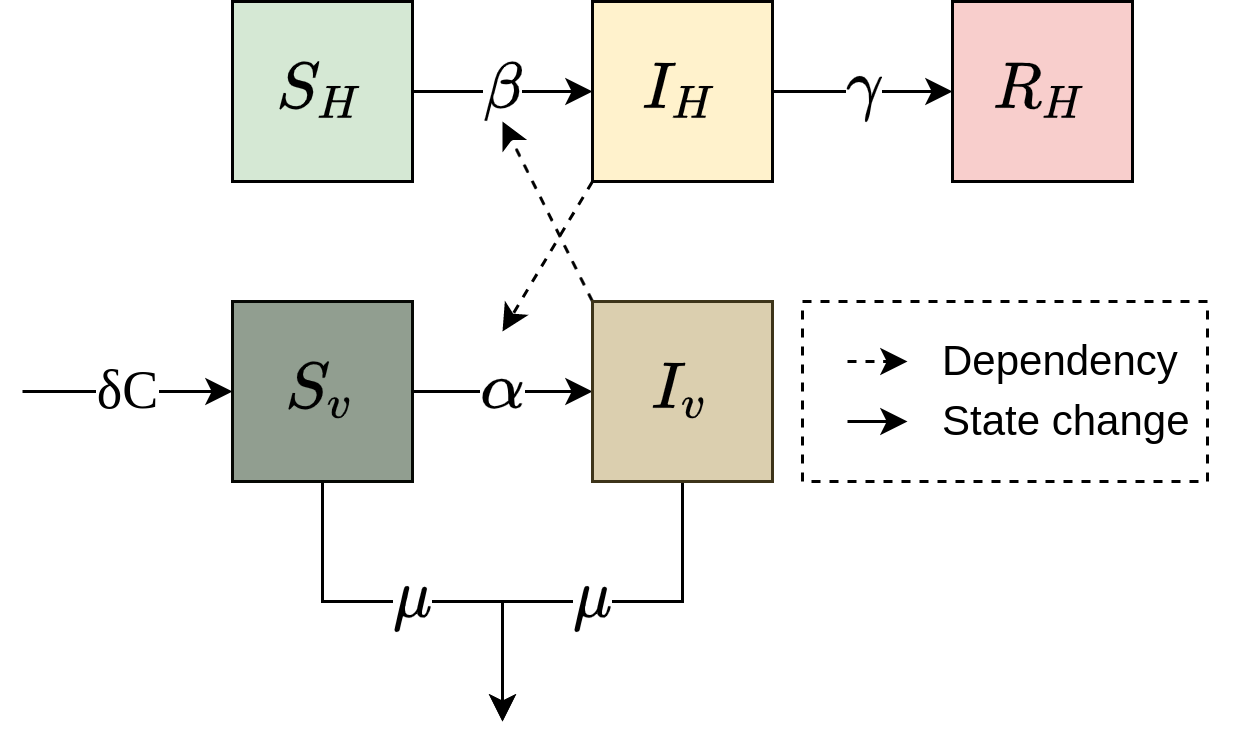
\includegraphics[width=0.9\textwidth]{Figures/Diagram.png}
    \caption[Diagram of the model]{Schematic representation of the model n
        \cref{eq:SIR_v}. Boxes
        are the compartments in which the population is divided, solid arrows
        represent
        changes in state (so transitions between compartments), and dashed
        arrows
        depict the crossed interaction between hosts and vectors.}
    \label{fig:model_diagram}
\end{figure}

\subsection{Preliminary analysis of the model} \label{sec:Prelimanalysis}

From \cref{eq:SIR_v} it is straightforward to verify that the population of
hosts remains constant over time, $N_H=S_H+I_H+R_H$, while the vector
population fulfils,
\begin{equation}\label{eq:dif_eq_Nv}
    \dot{N}_v=\dot{S}_v+\dot{I}_v=-\mu\parentesi{S_v+I_v}+\delta C=-\mu N_v
    + \delta C \ ,
\end{equation}
with solution,
\begin{equation}\label{eq:Nv_t}
    N_v(t)=\frac{\delta}{\mu}C +
    \parentesi{N_v(0)-\frac{\delta}{\mu}C}e^{-\mu t} \ .
\end{equation}
From \cref{eq:Nv_t} one can write the stationary value for the vector
population, $N_v^*$,
\begin{equation}
    N_v^*=\lim_{t\to\infty}N_v(t)=\frac{\delta}{\mu}C \ .
    \label{eq:asympt}
\end{equation}
Thus, if the initial population of vectors is below (above) the stationary
value, the vector population will grow (decrease) until it reaches the
stationary value. On the other hand, if $N_v(0)=N_v^*=\delta C/\mu$ the initial
population of vectors is already at the stationary state. The initial condition
for the vector population can be written in terms of its stationary value
\cref{eq:asympt}, $N_v(0)=fN_v^*$, where both $f<1$ and $f>1$ are possible, so
that one gets,
\begin{equation}\label{eq:Nv_t_fraction}
    N_v(t)=N_v^*\claudator{1+\parentesi{f-1}e^{-\mu t})} \ .
\end{equation}

We note that vector-borne disease models that assume constant vector
populations (e.g.\cite{Brauer2016}) can be recovered by setting $\delta=\mu$
and $C=N_v(0)$, so that any initial condition for the vector population is
stationary, i.e. $\dot{N}_v=0$ in \cref{eq:dif_eq_Nv} and $N_v(t)=N_v(0)$. We
note that our model describes populations with an asymptotic stationary vector
population and cannot describe periodic vector populations.

\section{Results} \label{sec:results}

%\subsection{The basic reproduction number for stationary vector populations}
\subsection{Epidemic threshold and disease dynamics}
\label{sec:R0statvp}

Let us start with the cases in which any initial condition for the vector
population is stationary  and the total vector population remains unchanged.
This will happen when the birth $\delta$ and death $\mu$ vector rates are
identical, independently on the initial condition of the vector population, or
the case in which the initial condition of the vector population is already at
its stationary value, $N_v(0)=N_v^*$, independently of the values of $\delta$
and $\mu$. In such a case, the initial disease free state of the model, given
by $I_H(0)=I_v(0)=0$, is a fixed point (equilibrium state) of the dynamical
system \cref{eq:SIR_v} independently of the other initial conditions for the
host and vector populations. This allows the definition of the basic
reproduction number, $R_0$, using standard methods such as linear stability
analysis or the Next-Generation Matrix (NGM) method \cite{Diekmann2010} (see
\cref{app:R0_standar_methods}).

In other cases, the total vector population will vary with time provided
that the initial condition, $N_v(0)$, is not identical to the asymptotic value
at large times, $N_v^*$. In these cases, an initial disease-free state is not
an equilibrium (fixed point) of the model. However, in the literature it is
customary to apply the standard techniques, i.e. NGM, to compute $R_0$ using
the vector population in the asymptotic state, that is the post-pandemic
disease-free equilibrium \cite{Martcheva2008, Lashari2011, Shah2013, Zhao2020,
    Esteva1998}.
The use of these methods is supported by the fact that the asymptotic
dynamics of the model converges to the dynamics of the subsystem where the
vector population is stationary \cite{Thieme1992,Thieme1995}. In both cases
the basic reproduction number is given by,
\begin{equation}\label{eq:R0_asympt}
    R_0=\frac{\beta\alpha}{\mu\gamma}\frac{S_H(0)}{{N_H}^2}N_v^* \ .
\end{equation}
As usual, $R_0$ accounts for the number of secondary infections produced by
an infected individual in one generation and controls the threshold behavior of
the model: for $R_0<1$ the epidemic dies out and for $R_0>1$ an outbreak
occurs. By one generation we refer to the typical time in which new infections
can be produced, being the generation time in our model,
\begin{equation}
    t_g=1/\gamma + 1/\mu\ .
    \label{eq:generationtime}
\end{equation}

Now we will show that \cref{eq:R0_asympt} is not always predictive about the
onset of the epidemic.
In \cref{fig:R0_check_stationary} the final size of the epidemic,
$R_{\infty}/N_H$, is plotted as a function of $R_0$, where $R_\infty$ is the
number of dead individuals at the end of the epidemic.
\cref{fig:R0_check_stationary}(a)-(d) show that \cref{eq:R0_asympt} does indeed
regulate the onset of an epidemic when the initial vector population is in its
stationary value or below it. This result is general and does not depend on the
time-scales of the system, $1/\gamma$ and $1/\mu$, and so all curves in these
panels behave similarly. In contrast, \cref{fig:R0_check_stationary}(e)-(f)
shows that \cref{eq:R0_asympt} does not predict the onset of epidemic outbreak
when the initial vector population is larger than the stationary value. Thus,
for $R_0<1$ (computed using  \cref{eq:R0_asympt}) severe outbreaks appear,
yielding mortalities even above 80\% of the total population. However, one can
observe that  as $\mu$ is increased, or $\gamma$ decreased, the predictive
power of \cref{eq:R0_asympt} is progressively recovered.

\begin{figure*}[t!]
    \centering
    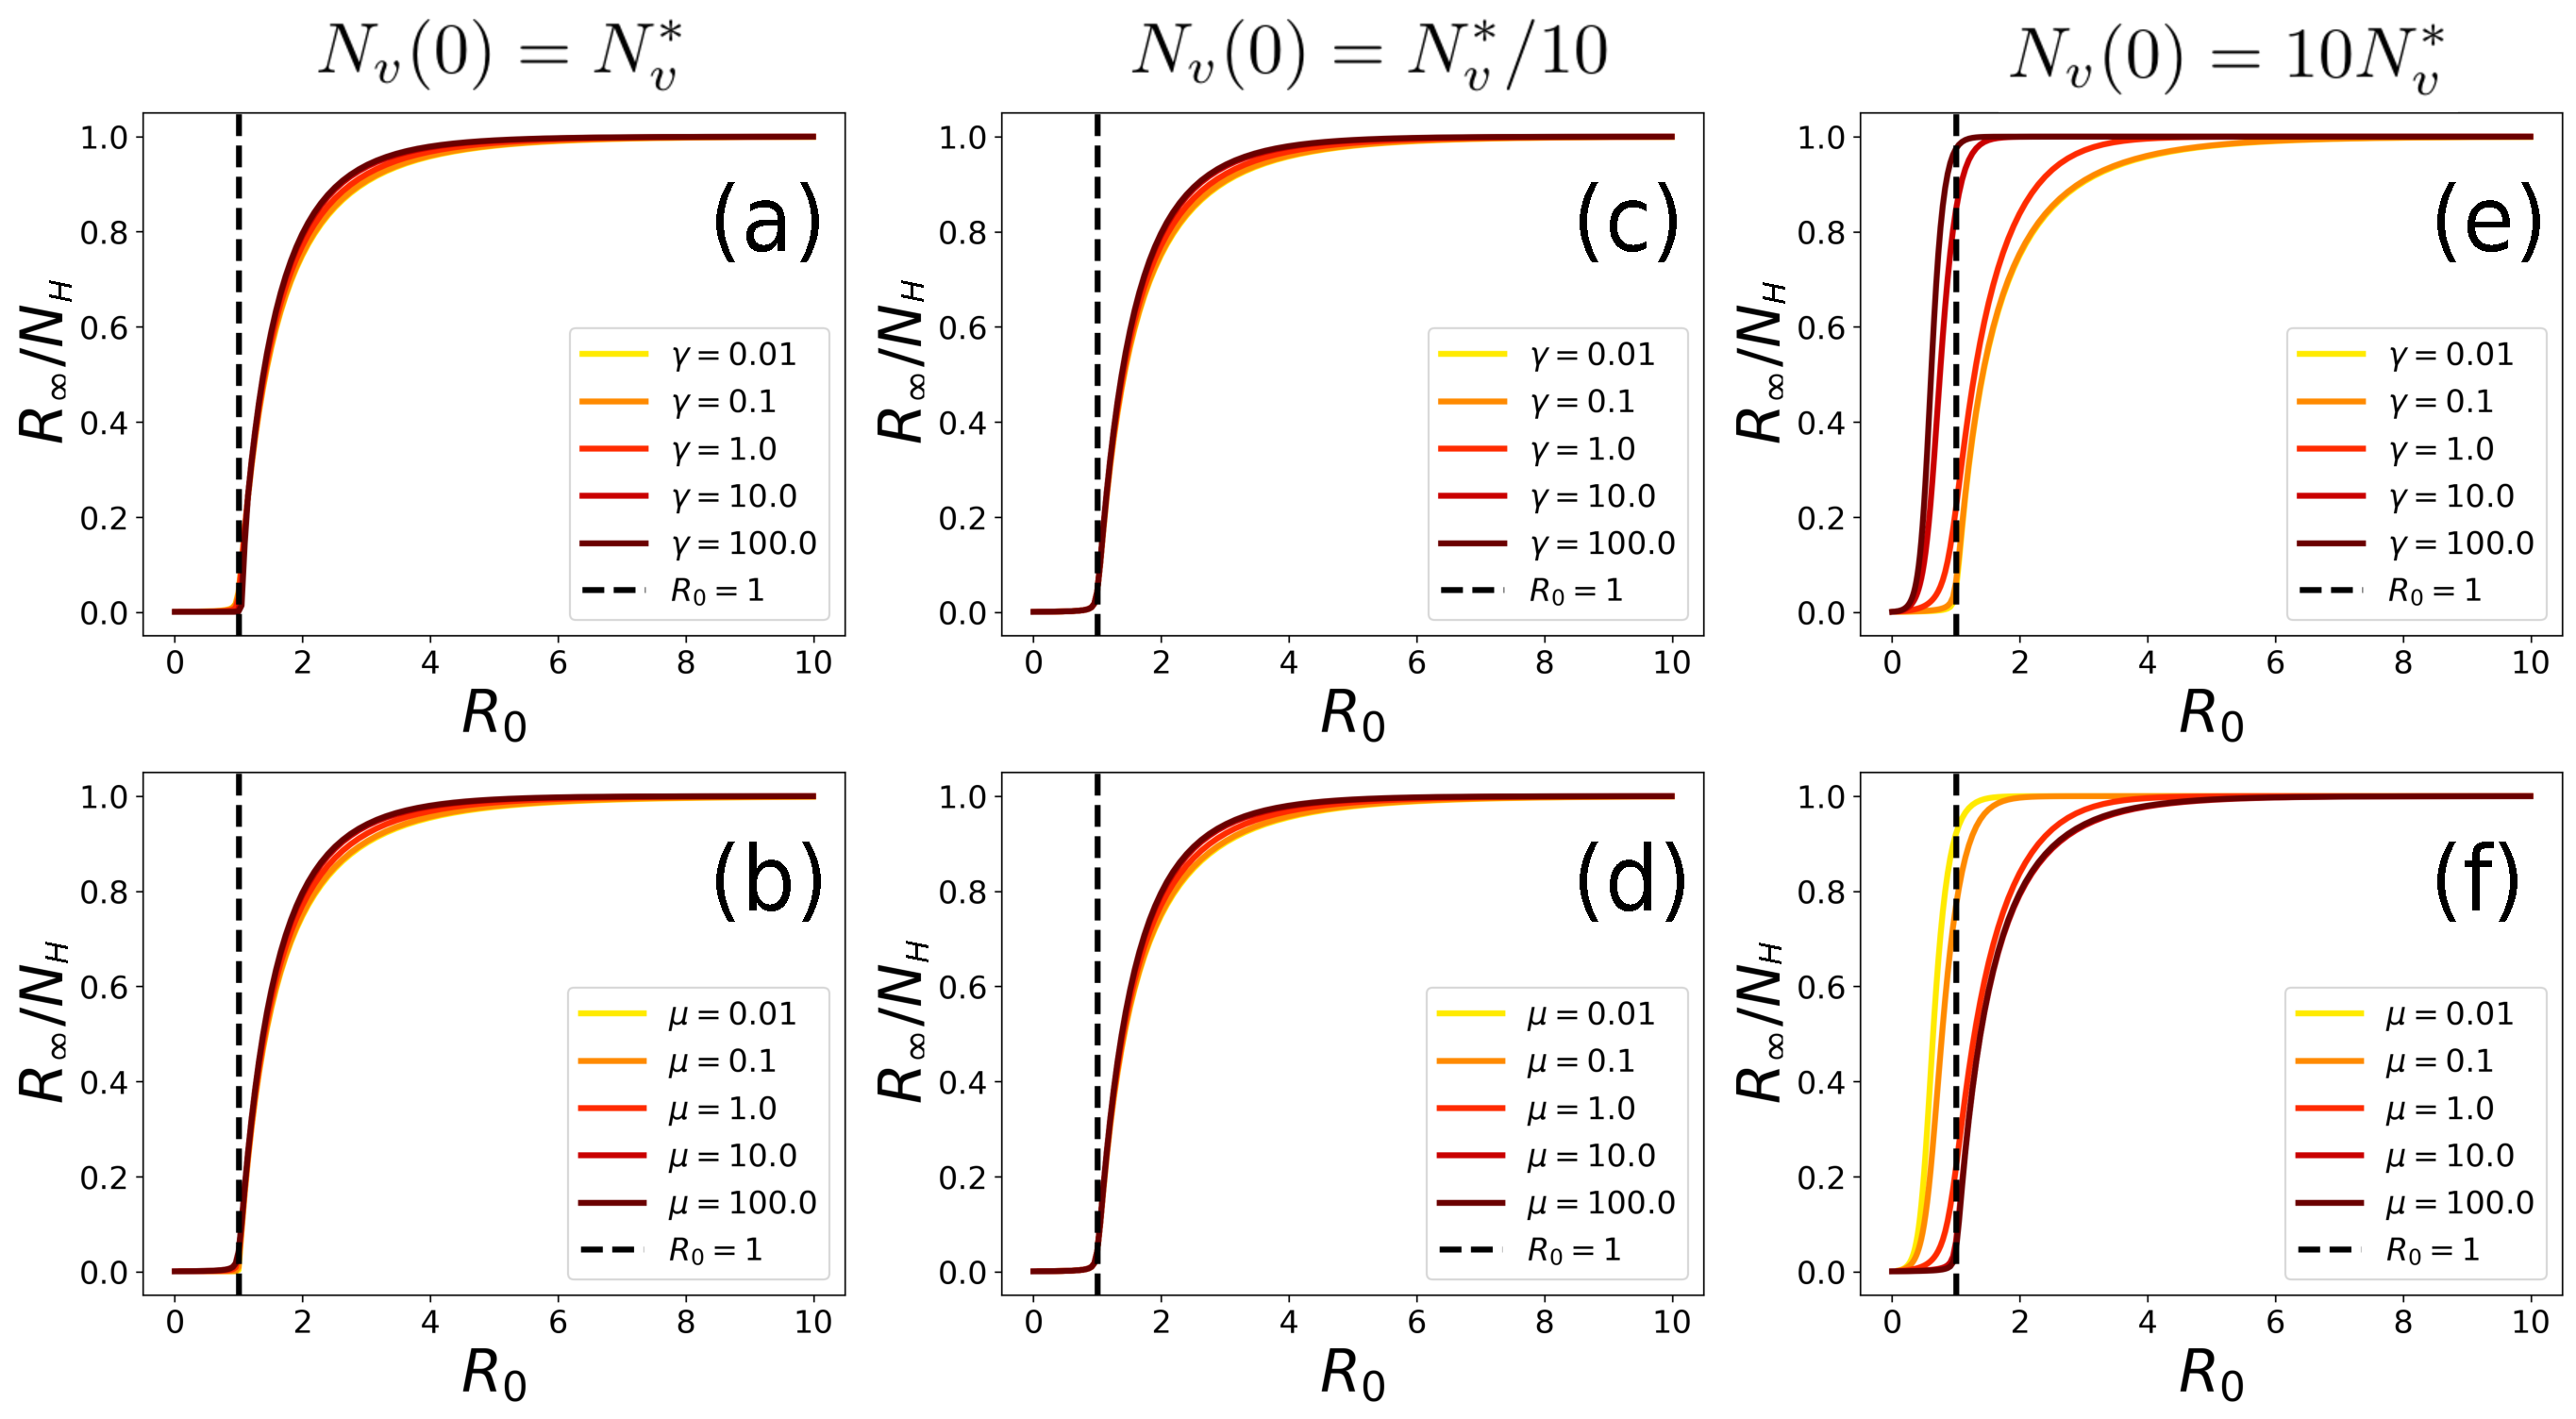
\includegraphics[width=\textwidth]{Figures/R0_check_stationary.pdf}
    \caption[
        Numerical verification of the predictive power of the
        stationary basic reproduction number
    ]{Numerical verification of the predictive	power of the basic
        reproduction number relation \cref{eq:R0_asympt}, by plotting the final
        size of
        the epidemic, $R_\infty/N_H$ as function of $R_0$. In panels (a),(b)
        the
        initial vector population is in the stationary value, in panels (c),(d)
        is
        below, $N_V^*/10$, and in panels (e),(f) above, $10 N_V^*$. Panels
        (a),(c),(e)
        show realisations for different $\gamma$ values with a fixed $\mu=1$
        baseline
        value. Panels (b),(d),(f) show realisations for different $\mu$ values
        with a
        fixed $\gamma=1$ baseline value.}
    \label{fig:R0_check_stationary}
\end{figure*}

Thus, only if the vector population reaches its stationary value before
infected hosts have produced new infections can the onset of an epidemic be
characterized by \cref{eq:R0_asympt}. Let us discuss separately the cases $f>1$
and $f<1$, with $N_v(0)=fN_v^*$, namely when the initial vector population is
above and below its stationary value, this is, decaying and growing vector
populations towards the asymptotic state.

If $f>1$ \cref{eq:Nv_t_fraction}, the time to approach the stationary
value, $t^*$, is,
\begin{equation}
    \parentesi{1+\epsilon}N_v^*=N_v^*\claudator{1+(f-1)e^{-\mu t^*}} \ ,
\end{equation}
where $\epsilon\to 0$ is a small parameter controlling the amount by which
the vector population differs from its asymptotic value at time $t^*$. Thus,
the time to approach the stationary value, with precision $\epsilon$, is given
by
\begin{equation}
    t^*=-\frac{1}{\mu}\ln(\frac{\epsilon}{f-1})=
    \frac{1}{\mu}\abs{\ln{\frac{\epsilon}{f-1}}}
    \ ,
\end{equation}
where the last equality assumes that the small parameter $\epsilon$
satisfies $\epsilon<(f-1)>0$.

If the vector population reaches its stationary value before infected hosts
have had time to generate new infections then $R_0$ as determined from
\cref{eq:R0_asympt} is a good prediction of the onset for an epidemic, what is
equivalent to the condition that $t^*$ is much smaller than the hosts
infectious period, $t^*\ll1/\gamma$,
\begin{equation}\label{eq:timescales_condition}
    \frac{1}{\gamma} \gg \frac{1}{\mu}\abs{\ln{\frac{\epsilon}{f-1}}} \quad
    \textrm{or} \quad \frac{\mu}{\gamma}\gg\abs{\ln{\frac{\epsilon}{f-1}}}
    \ .
\end{equation}
Otherwise, \cref{eq:R0_asympt} will not be predictive of the epidemic
onset, and as shown in \cref{fig:R0_check_stationary}(e-f) one may have
outbreaks with a substantial final size with $R_0<1$.\\

In the case of growing vector populations, $f<1$, if $R_0<1$ an outbreak
cannot occur at all, because $R_0$ is calculated with the asymptotic
population, $N_v^*$, that is larger that the vector population at any finite
time, $N_v(t)<N_v^* \ \forall t$, and so the threshold condition is never
attained. In the $R_0>1$ case the behaviour will be richer, and it will depend
on the initial condition, $N_v(0)$. One can define an instantaneous basic
reproductive number,
\begin{equation}\label{eq:R0i}
    R_0^{(i)}(t)=\frac{\beta\alpha}{\mu\gamma}\frac{S_H(0)}{{N_H}^2}
    N_v(t)=R_0\frac{N_v(t)}{N_v^*} \ ,
\end{equation}
using $N_v(t)$ instead of $N_v^*$, with $R_0^{(i)}(t)<R_0 \ \forall t$
because the vector population grows. In particular, if $R_0^{(i)}(0)>1$ there
will be an outbreak occurring for short times, and the population of infected
hosts will start growing. If instead, $R_0^i(0)<1$, and as $R_0>1$ with $R_0$
being calculated with the asymptotic state, there must be an intermediate time,
say $t_D$, for which $R_0^{(i)}(t_D)=1$. Thus, from $t>t_D$ an outbreak will
occur, not initially but after a finite time, that induces a delay in the
outbreak, and the infected host population will start growing.

The difference between the original and the delayed dynamics stems from the
waiting time to reach $R_0^{(i)}=1$, $t_D$, plus the non-linear effect
associated to a new initial condition for the epidemic outbreak at $t_D$. Thus,
in the case that $R_0>1$ and $R_0^{(i)}(0)<1$, from \cref{eq:R0i} and
\cref{eq:Nv_t_fraction} we can analytically approximate the delay as the time
needed to reach $R_0^{(i)}(t_D)=1$,
\begin{equation}
    {1+(f-1)e^{-\mu t_D}}=\frac{1}{R_0} \ ,
\end{equation}
which yields the relation,
\begin{equation}\label{eq:delay}
    t_D=-\frac{1}{\mu}\ln\claudator{\frac{1-R_0}{\parentesi{f-1}R_0}}\ ,
\end{equation}
where the argument of the logarithm is always positive because $R_0>1$ and
$f<1$. \cref{eq:delay} is only valid if $f<1/R_0$, for $R_0^{(i)}(0)=f R_0<1$,
as if otherwise $R_0^{(i)}>1$ the outbreak would already occur initially.

From \cref{eq:delay} one can see that when the initial vector population
is far enough from its stationary value, $f\rightarrow 0$, the delay saturates
to a constant value, instead of increasing. This is,
%    \begin{equation}
%        \lim_{f\to0}t_D= %-\frac{1}{\mu}\ln(\frac{R_0-1}{R_0})=\frac{1}{\mu}\ln(\frac{R_0%}{R_0-1}) \ .
%        \label{eq:limitd}
%    \end{equation}
\begin{equation}
    \lim_{f\to0}t_D=\frac{1}{\mu}\ln(\frac{R_0}{R_0-1}) \ .
    \label{eq:limitd}
\end{equation}
In addition, for increasing values of the basic reproduction number, $R_0$,
the delay tends to vanish, and from \cref{eq:limitd}. This is,
\begin{equation}
    \label{eq:limit_tD_infty}
    \lim_{R_0\to\infty}t_D=\frac{1}{\mu}\ln(1)=0\ ,
\end{equation}
where the limit $f\rightarrow 0$ is taken simultaneously to guarantee that
$R_0^{(i)}(0)=f R_0<1$. On the other hand the delay, $t_D$, scales with the
vectors lifetime,
\begin{equation}
    t_D\sim\frac{1}{\mu}=\tau_v \ .
\end{equation}

\cref{fig:delay}(a) shows an example of the time delay caused in the hosts
dynamics when the vector population grows from an initial condition far from
the stationary value. In \cref{fig:delay}(b) we can qualitatively observe that
all the predicted properties of the delay are fulfilled, namely, the time delay
saturates for low $f$ values and decreases with increasing $R_0$. Although the
analytical expression (black dashed line) is clearly not exact due to nonlinear
effects, \cref{eq:delay} captures the basic trends of the time delay, $t_D$.
This is clear from \cref{fig:delay}(c), that shows that the delay scales with
$1/\mu$ and in \cref{fig:delay}(d) that shows that the delay tends to $0$ in
the limit $R_0\rightarrow\infty$, in agreement with the prediction of
\cref{eq:limit_tD_infty}.

\begin{figure}[H]
    \centering
    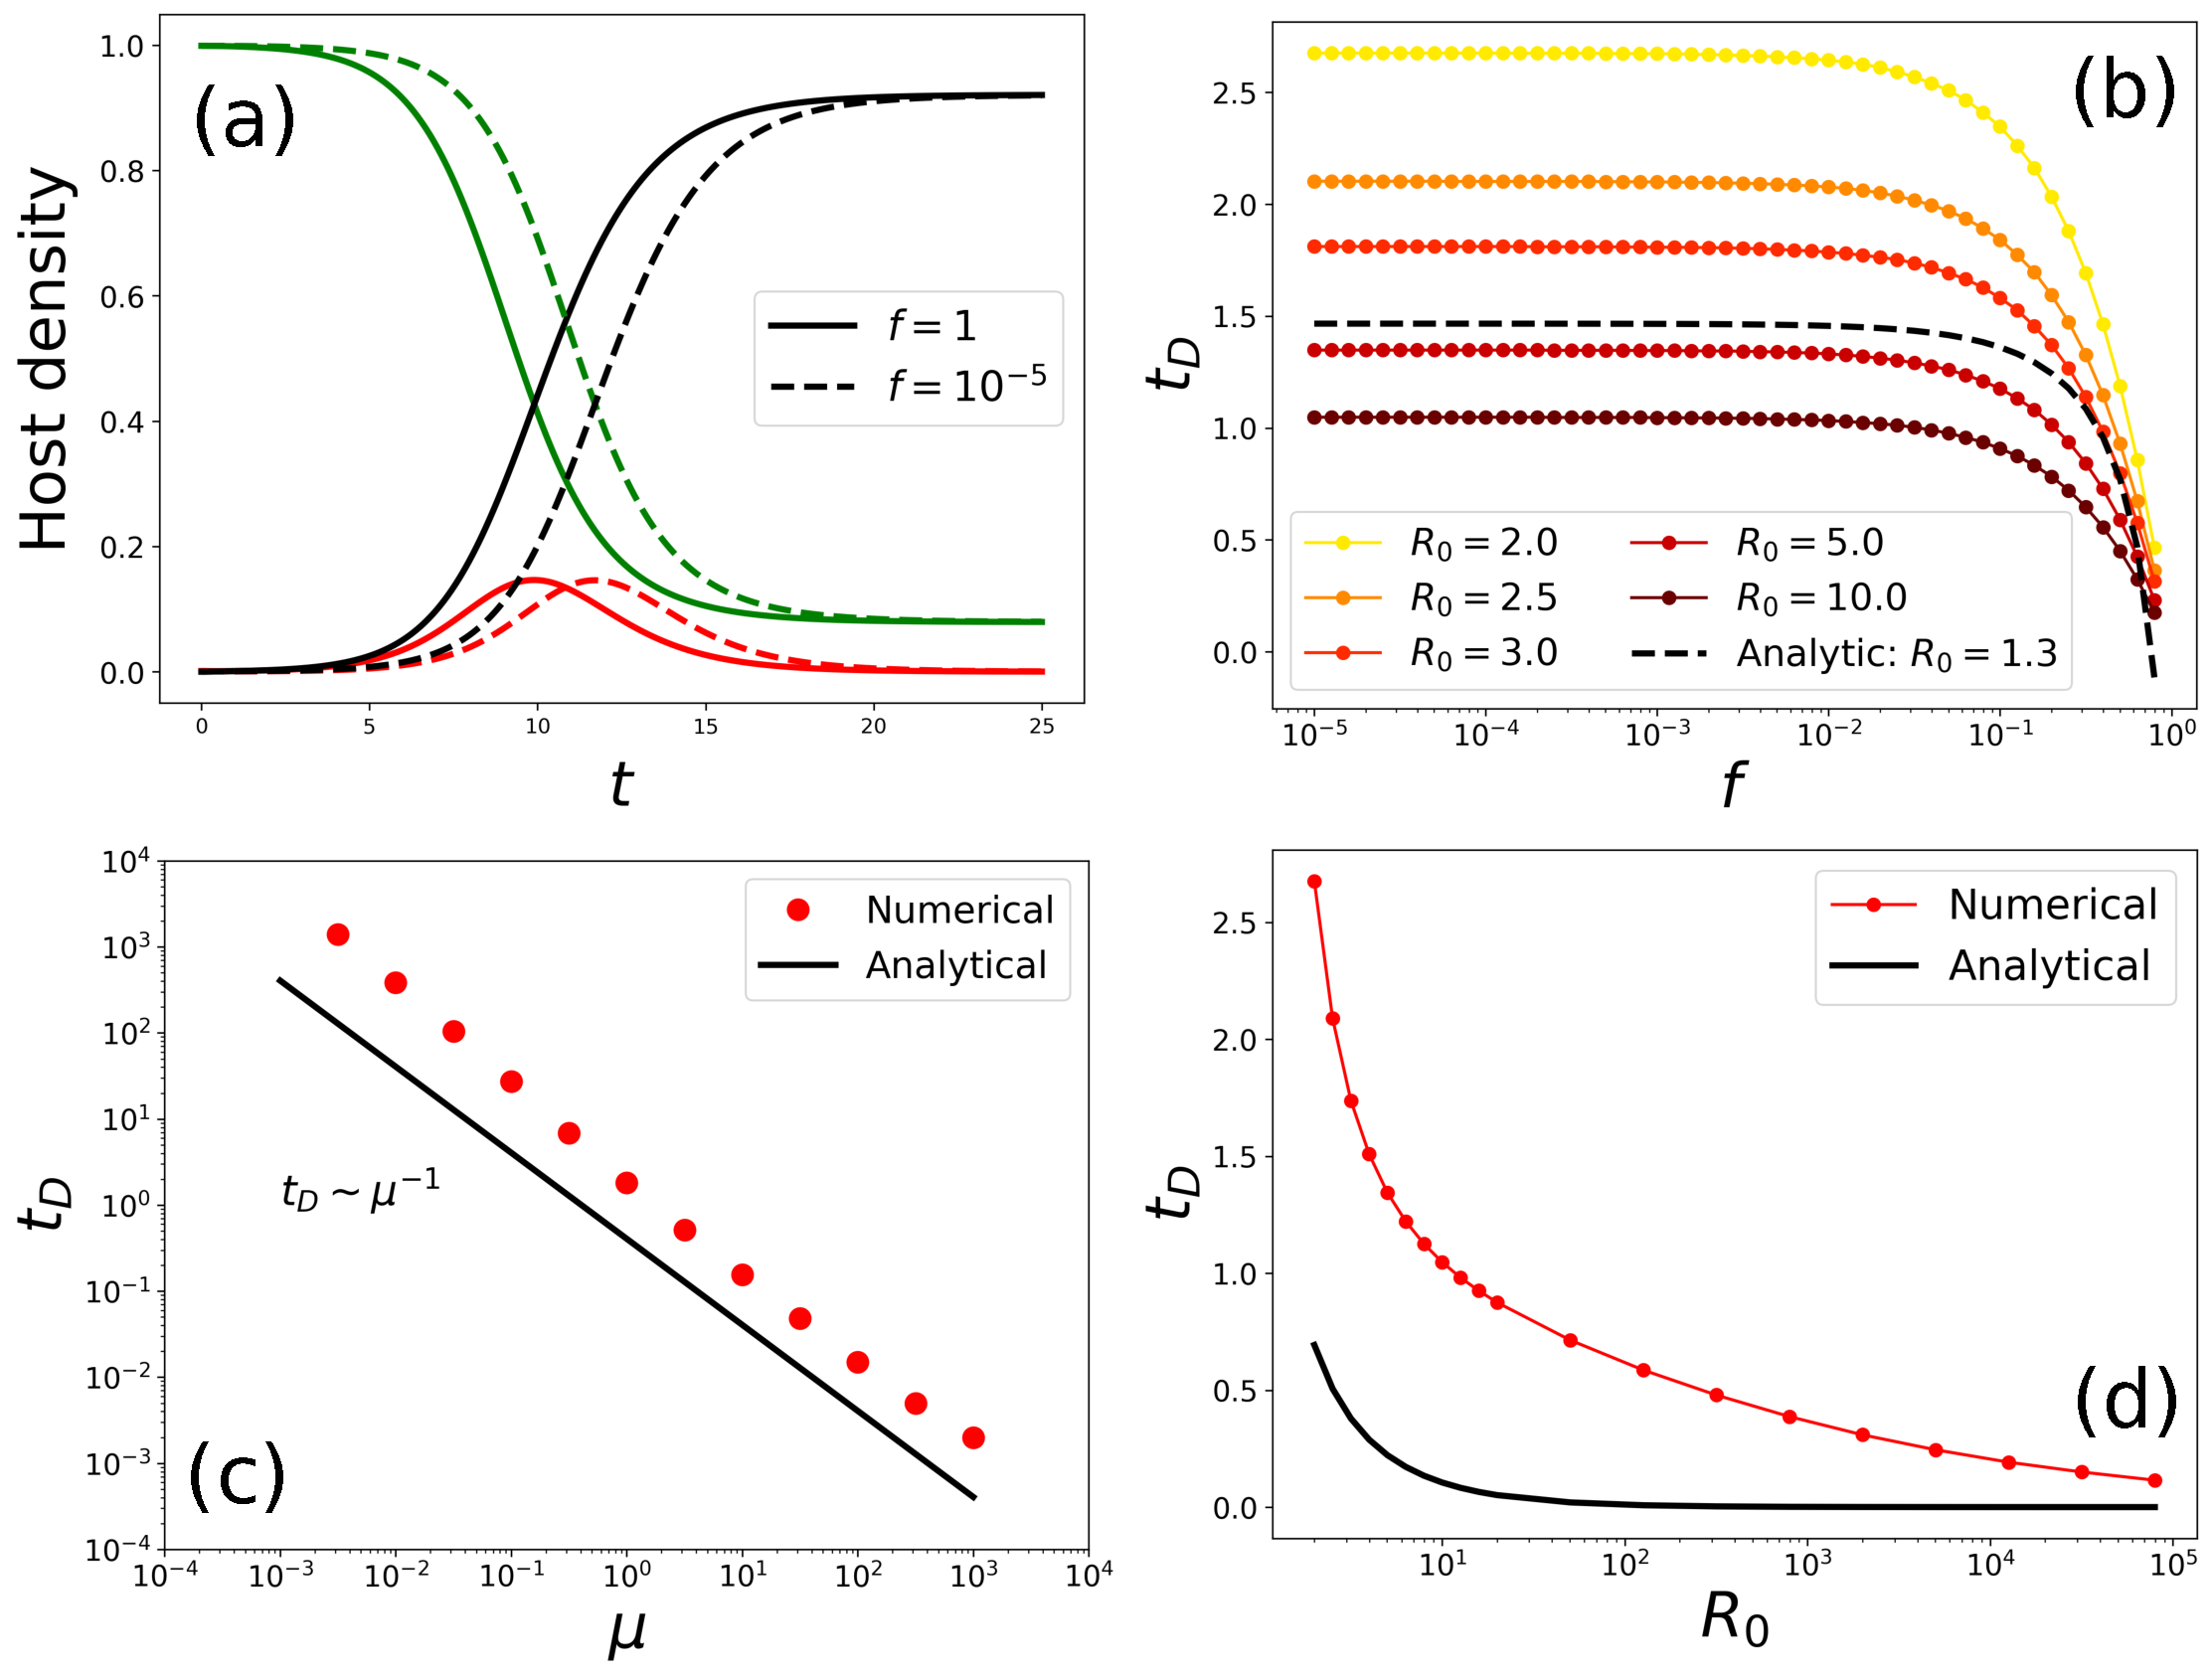
\includegraphics[width=0.8\textwidth]{Figures/delay.pdf}
    \caption[Numerical study of the delay induced by growing vector
    populations]{Numerical study of the delay induced by growing vector
    populations. (a) Comparison of hosts dynamics for a stationary vector
    population ($f=1$) and a growing vector population ($f=10^{-5}$). (b) Time
    delay as function of $f$ for different values of the basic reproduction
    number
    $R_0$. (c) Time delay as function of the vector natural death rate. (d)
    Time
    delay as function of the basic reproduction number, $R_0$, with
    $f=10^{-5}$.}
    \label{fig:delay}
\end{figure}

\subsection{The basic reproduction number for non-stationary vector
    populations}

As shown in the previous section, traditional methods to compute the basic
reproduction number fail in the case of epidemic models with decaying vector
populations, $f>1$, unless the time scale of vector population fulfils the
strong inequality condition \cref{eq:timescales_condition}, as illustrated in
\cref{sec:R0statvp}. Here we introduce an effective, average definition of
$R_0$, useful to predict the epidemic onset for vector-borne diseases with
decaying vector populations, i.e. the case where traditional methods fail. It
is defined as the \textit{average} number of infections produced by an infected
individual in \textit{one generation} \cref{eq:generationtime},
\begin{equation}\label{eq:R0_non_stationary}
    \overline{R_0}=\avg{R_{0}^{i}(t)}\Big\rvert\limitss{0}{t_g}=
    R_0\claudator{1-\frac{1}{\tau}\parentesi{f-1}
        \parentesi{e^{-\tau}-1}}=R_0\cdot\mathcal{F}
\end{equation}
where $\tau=1+\mu/\gamma$ and $\mathcal{F}$ accounts for the effect of the
decaying vector population on the stationary $R_0$ (see
\cref{app:R0_non_stationary} for the full derivation of
\cref{eq:R0_non_stationary}).

A first observation is that $\overline{R_0}>R_0$ always (for $f>1$). This
stems from the fact that $\tau=1+\mu/\gamma>1$, so that $e^{-\tau}-1<0$, and
$f-1>0$, which yields $\mathcal{F}>1$. This discussion unravels why standard
methods fail to predict the onset of an epidemic under decaying vector
populations. Another important point is that if $\mu/\gamma\gg 1$, which
implies $\tau\gg1$,
\begin{equation}
    \lim_{\tau\gg1}\mathcal{F}=\lim_{\tau\gg1}\claudator{1-\frac{1}{\tau}
        \parentesi{f-1}\parentesi{e^{-\tau}-1}}=1+\frac{f-1}{\tau}\
    ,
\end{equation}
and if furthermore $\tau\sim\frac{\mu}{\gamma}\gg (f-1)$ then
$\mathcal{F}\to 1$ and $\overline{R_0}\to R_0$. This is in agreement with the
discussion in \cref{sec:R0statvp} showing that the $R_0$ computed from standard
methods works if $\mu\gg\gamma$.

\begin{figure}[H]
    \centering
    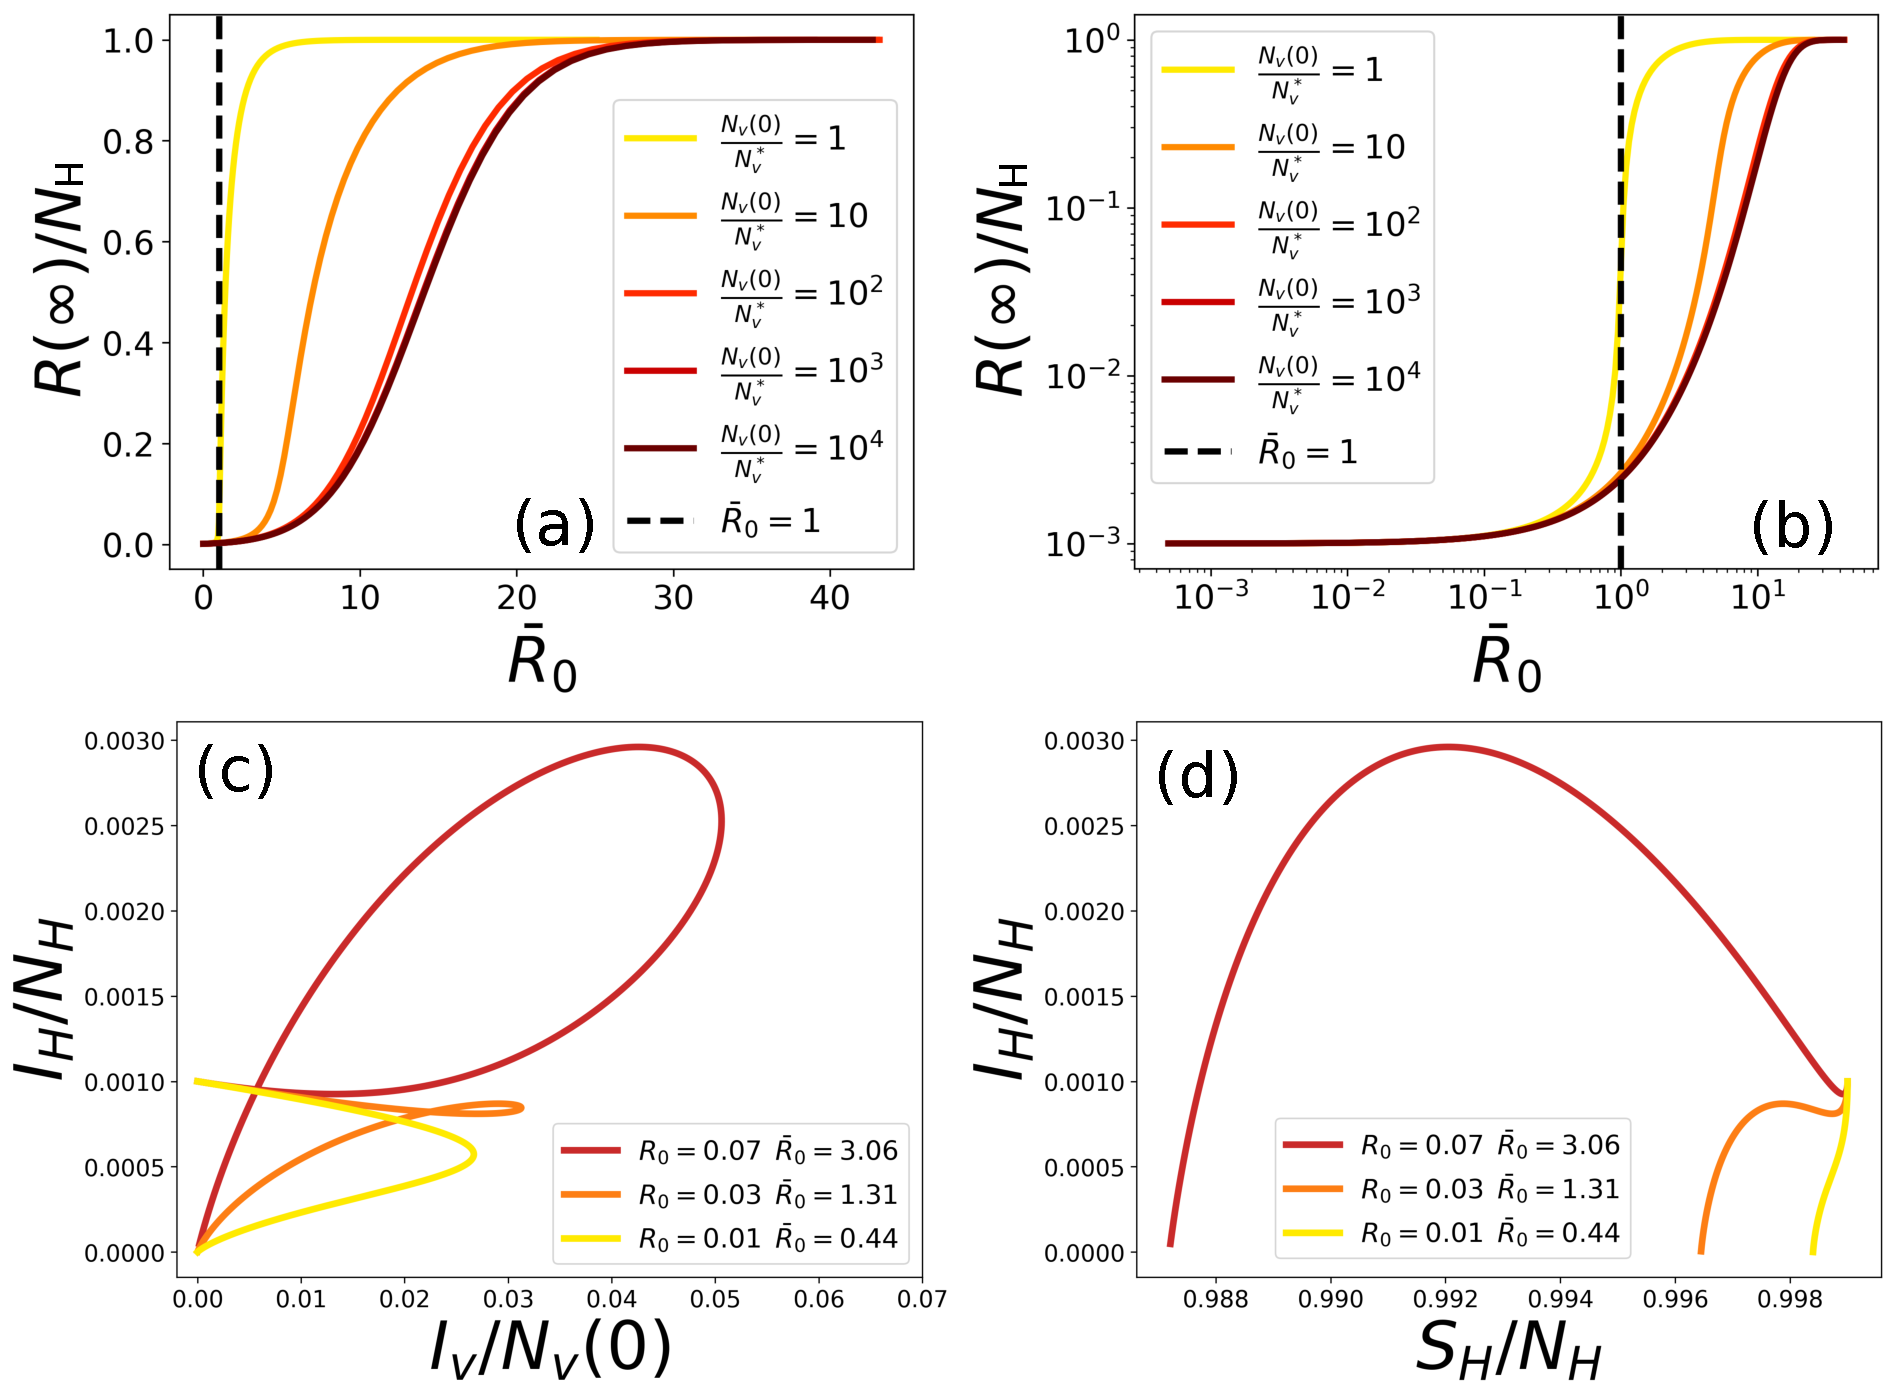
\includegraphics[width=0.8\textwidth]{Figures/R0_check_mean_value.pdf}
    \caption[Numerical verification of the expression for the non-stationaty
        basic reproduction number]{Numerical verification of the expression for
        the basic reproduction number for vector-borne diseases with decaying
        vector populations \cref{eq:R0_non_stationary}. Final size of the
        epidemic as a function of the basic reproduction number in panels: (a)
        linear scale; (b) logarithmic scale. Phase space trajectories in
        panels: (c) $I_H/N_H$ vs $I_v/N_v(0)$ and (d) $I_H/N_H$ vs $S_H/N_H$,
        where an initial condition $I_H(0)/N_H=0.01, S_H(0)/N_H=0.99$ and
        $I_v(0)/N_V(0)=0$ has been used for the $3$ cases.
        $\mu=\gamma$ has been used in all the simulations.}
    \label{fig:R0_check_mean_value}
\end{figure}

\cref{fig:R0_check_mean_value}(a-b) contrasts numerically the validity of
\cref{eq:R0_non_stationary} to predict the final size of the epidemic as a
function of the general basic reproduction number, $\overline{R_0}$, in linear
and logarithmic scale, respectively. We observe that, independently of the
initial condition of vectors, the outbreak occurs for $\overline{R_0}>1$.
However, we may notice that for large values of the initial condition of
vectors the final size of the epidemic grows more slowly, so that larger values
of $\overline{R_0}$ are needed to produce a proper outbreak. This can be
explained by the fact that for $\overline{R_0}$ slightly above the threshold,
$\overline{R_0}=1$, and large values of $f=N_v(0)/N_v^*$, infections are
produced only in the transient period of the dynamics, as $R_0<1$. This is,
while the vector population is decaying to its stationary value, the vectors
are able to produce new infections, but once the vector population reaches the
stationary value, the epidemics stops. This transmission mechanism is radically
different to that of vector-borne diseases with stationary vector populations
in which the pre-pandemic disease-free state is an equilibrium of the system.
The phase-space plots in \cref{fig:R0_check_mean_value}(c-d) show that the
time-averaged basic reproduction number $\overline{R_0}$ is able to accurately
predict the conditions under which the infected host population will grow, in
contrast with $R_0$ computed in the post-pandemic fixed point. In essence, for
$\overline{R_0}>1$ the infected host population, $I_H$, grows before reaching
the absorbing state, $I_H=I_v=0$, while for $\overline{R_0}<1$ the infected
host population is monotonically decreasing. We note that
\cref{eq:R0_non_stationary} is similar to the time-averaged basic reproduction
number presented in \cite{Wesley2009} for the periodic case, which is a
first-order approximation to the \textit{true} basic reproductive number
\cite{Bacaer2006}.

\subsection{Fast-slow approximation}

The original $5$-D \cref{eq:SIR_v} model is certainly not amenable to
mathematical analyses due to its high phase-space dimensionality and the fact
that it depends on $4$ parameters. Moreover, in a real-case application, if the
parameters conforming the model are not known, the model could suffer from
parameter unidentifiability. However, some approximations can be performed to
reduce the mathematical complexity of the model, as for instance a fast-slow
(or adiabatic) approximation.

If the time-scale of the vector population evolution is much faster than
that of the infected hosts, what is expected to be a good approximation in many
practical cases, the vector population will almost instantaneously adapt to its
stationary value. Thus, if $1/\mu\ll1/\gamma$, or equivalently if
$\gamma/\mu\ll1$, we can rewrite the time derivative of the vector infected
population as
\begin{equation}
    \epsilon\dot{I}_v=\frac{\alpha}{\mu}S_v\frac{I_H}{N_H} - I_v \ ,
\end{equation}
where time has been re-scaled to $t'\to\gamma t$ and $\epsilon=\gamma/\mu$
is a small parameter. Then, $\dot{I_v}$ can be neglected and the infected
vector population can be obtained from the relationship,
\begin{equation}\label{eq:Iv_timescale_approx}
    I_v\approx\frac{\alpha}{\mu}\frac{S_v I_H}{N_H} \ .
\end{equation}

\begin{figure}[H]
    \centering
    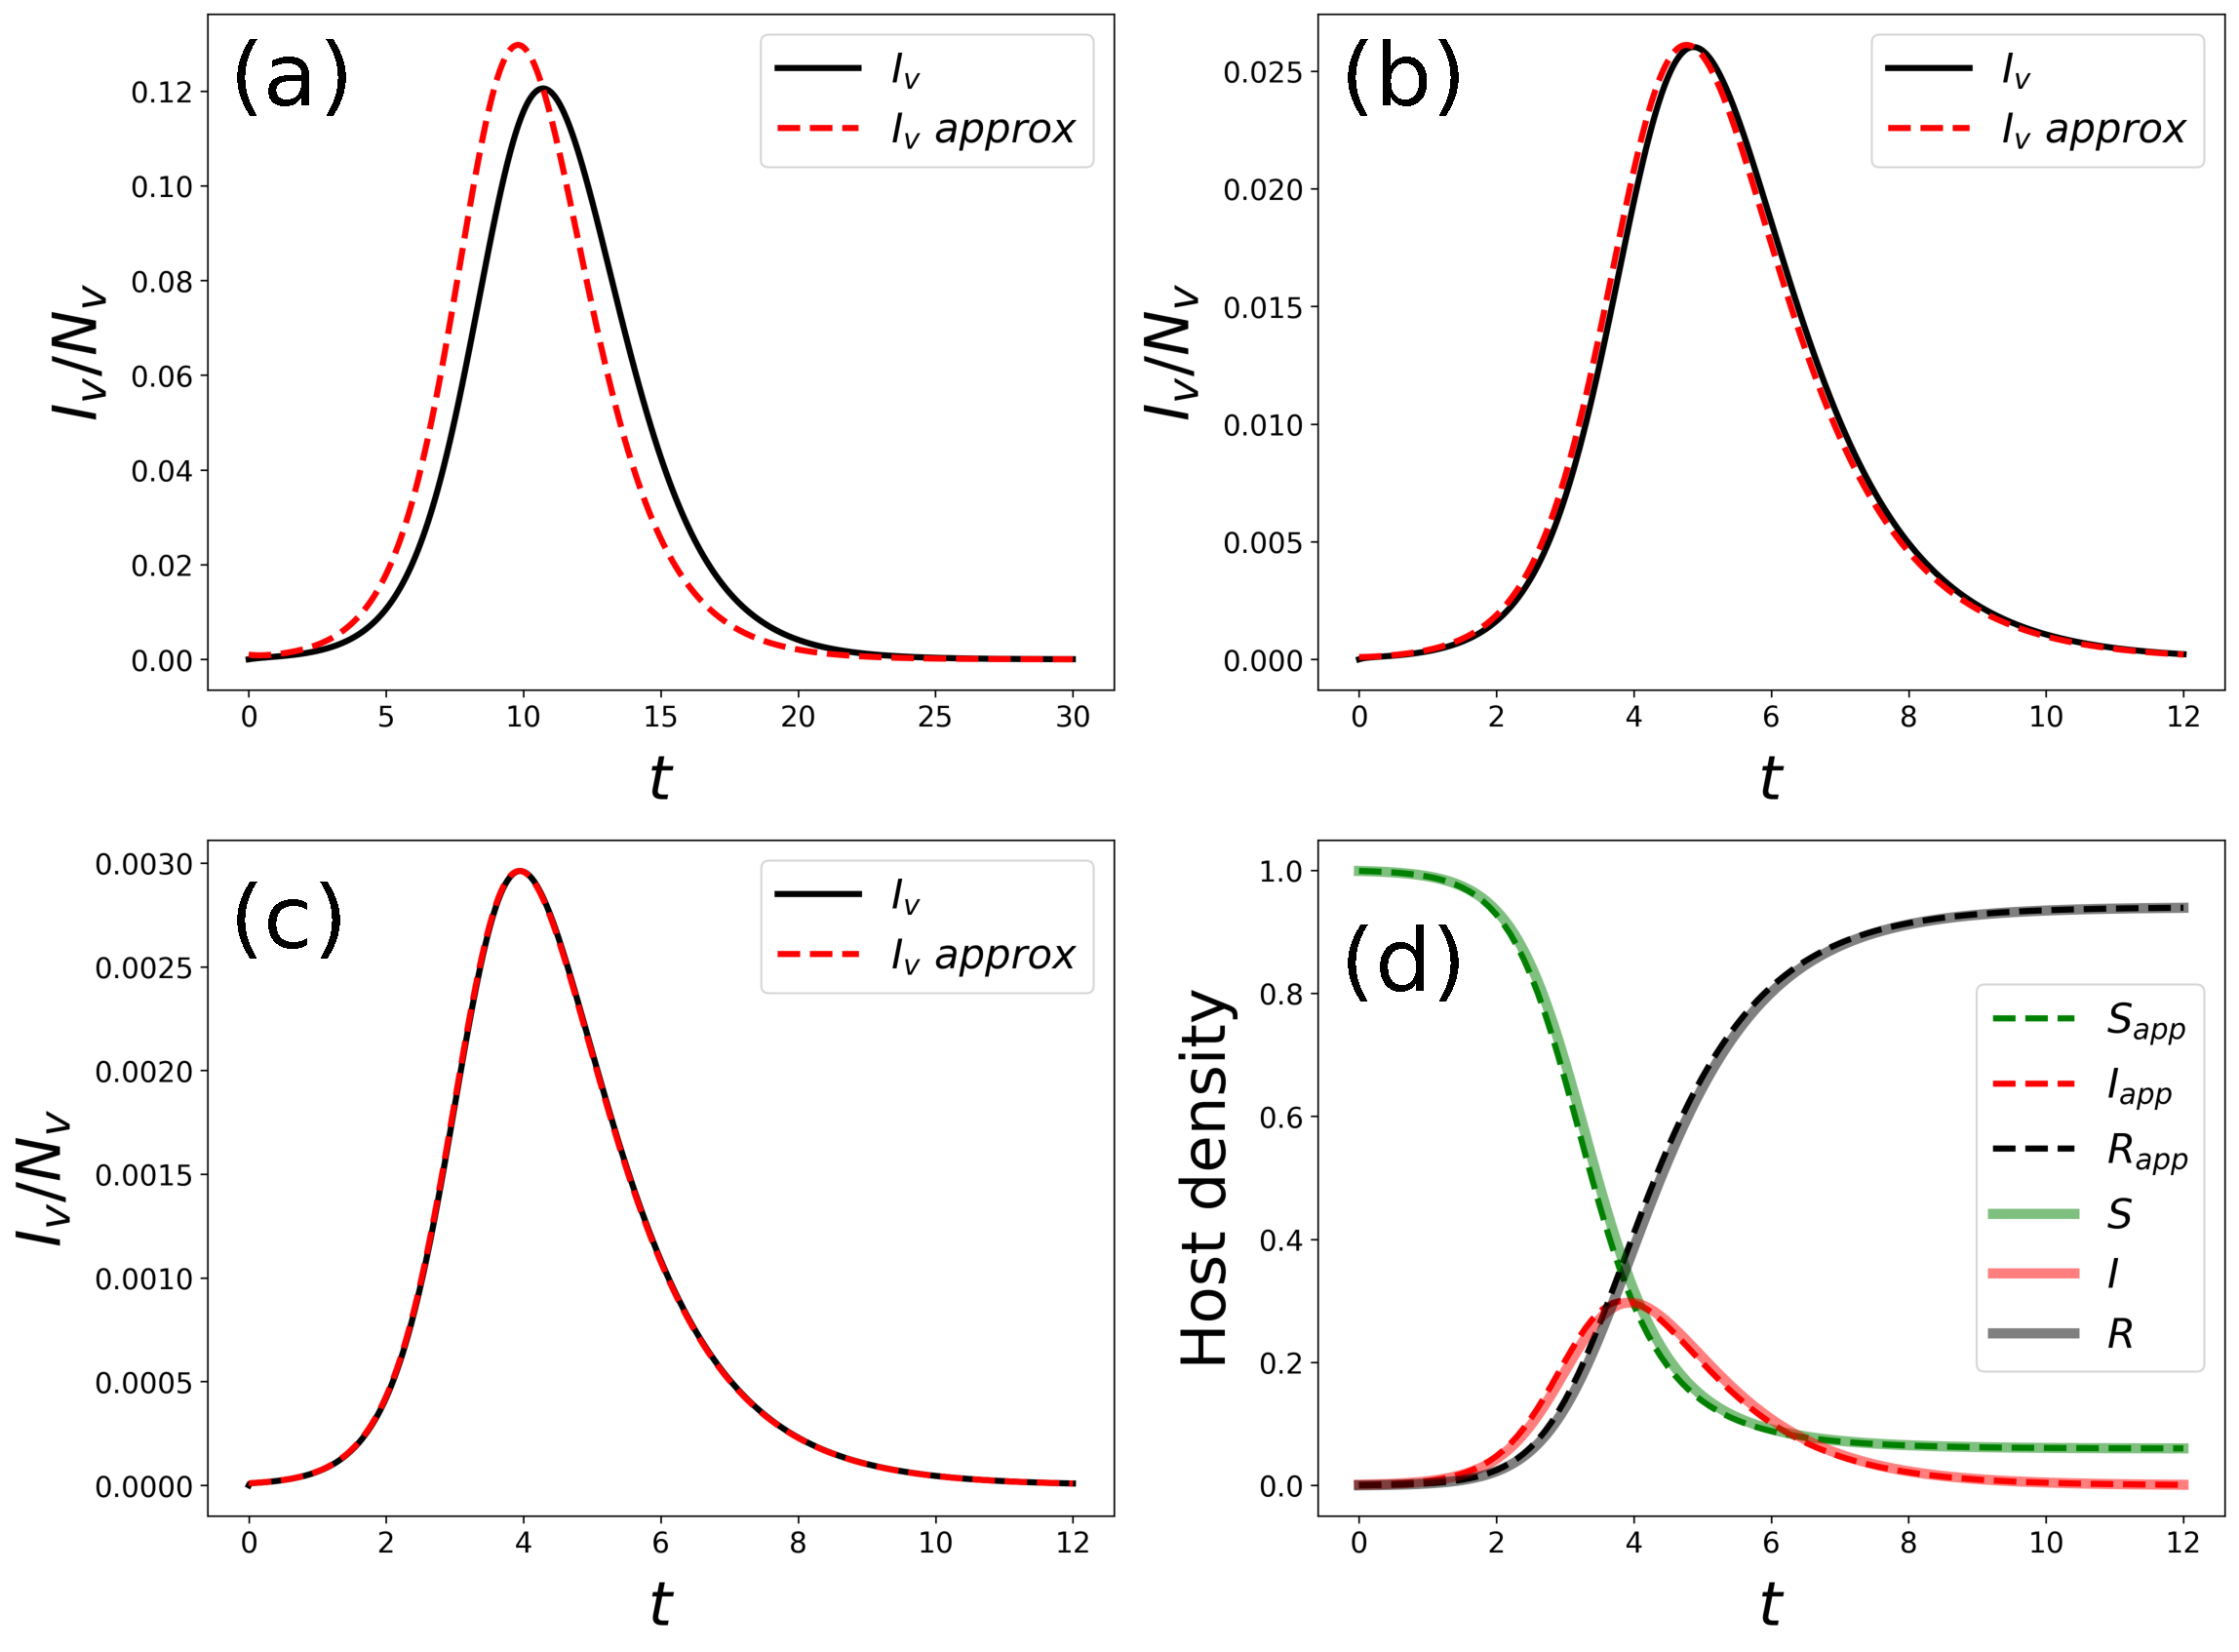
\includegraphics[width=0.8\textwidth]{Figures/Timescale_approx.pdf}
    \caption[Numerical verification of the time-scale approximation]{Numerical
        verification of the time-scale approximation
        (\cref{eq:Iv_timescale_approx}) with $N_H=100$, $\alpha=\gamma=1$.
        $\beta$ is
        chosen such that $R_0=3$. (a) $\mu=1$, (b) $\mu=10$, (c) $\mu=100$.
        Panel (d)
        shows a comparison between the approximate and original models for the
        parameters used in (c), where the approximated models is expected to
        represent
        well the original one.}
    \label{fig:timescale_approx}
\end{figure}

Substituting \cref{eq:Iv_timescale_approx} into the original system
\cref{eq:SIR_v} and the identity $N_v(t)=S_v(t)+I_v(t)$, while considering that
the conditions for which the time-scale approximation is valid, $\mu\gg\gamma$,
imply that the vector population will reach its stationary value almost
instantaneously, so that $N_v(t)\approx N_v^*$, we obtain the following reduced
system,
\begin{equation}\label{eq:SIR_like}
    \begin{aligned}
        \dot{S}_H & =-\beta'\frac{S_H I_H}{\lambda N_H + I_H}            \\
        \dot{I}_H & =\beta'\frac{S_H I_H}{\lambda N_H + I_H}- \gamma I_H \\
        \dot{R}_H & =\gamma I_H \ ,
    \end{aligned}
\end{equation}
where $\beta'=\beta N_v^*/N_H$ and $\lambda=\mu/\alpha$.

Moreover, if $f\neq1$ the above mentioned timescales relationship
must fulfil
$\displaystyle\frac{\mu}{\gamma}\gg\abs{\ln{\frac{\epsilon}{f-1}}}$ (cf.
\cref{eq:timescales_condition}) and not only
$\displaystyle\frac{\mu}{\gamma}\gg 1$. It is important to notice that the
presence of direct host to host transmission would simply re-scale the
coefficient $\beta'$, and the SIR reduction \cref{eq:SIR_like} would keep its
validity.

In \cref{fig:timescale_approx} we numerically verify the validity of the
presented fast-slow approximation. As expected, we observe that the
approximation breaks down for $\mu\sim\gamma$ (\cref{fig:timescale_approx}(a)),
while as
$\mu$ becomes larger than $\gamma$ the approximation improves
\cref{fig:timescale_approx}(b) and it becomes quantitative when $\mu\gg\gamma$,
\cref{fig:timescale_approx}(c). Finally, we show in
\cref{fig:timescale_approx}(d) a comparison between the dynamics of the hosts
using both the original and the approximated model using the same parameters
than in \cref{fig:timescale_approx}(c), where the results of both models are
expected to converge.

\subsection{Reduction to a SIR model}

In addition to the previous condition, $\gamma/\mu\ll1$, if one has that
$\lambda N_H \gg I_H$ also holds (which is indeed plausible in this limit)
\cref{eq:SIR_like}, then the model can be written as a standard SIR model,
\begin{equation}\label{eq:SIR}
    \begin{aligned}
        \dot{S}_H & =-\beta_{eff}\frac{S_HI_H}{N_H}            \\
        \dot{I}_H & =\beta_{eff}\frac{S_HI_H}{N_H}- \gamma I_H \\
        \dot{R}_H & =\gamma I_H \ ,
    \end{aligned}
\end{equation}
where $\displaystyle\beta_{eff}=\frac{\beta'}{\lambda}=\frac{\beta\alpha
        N_v^*}{\mu N_H}$.

\begin{figure}[H]
    \centering
    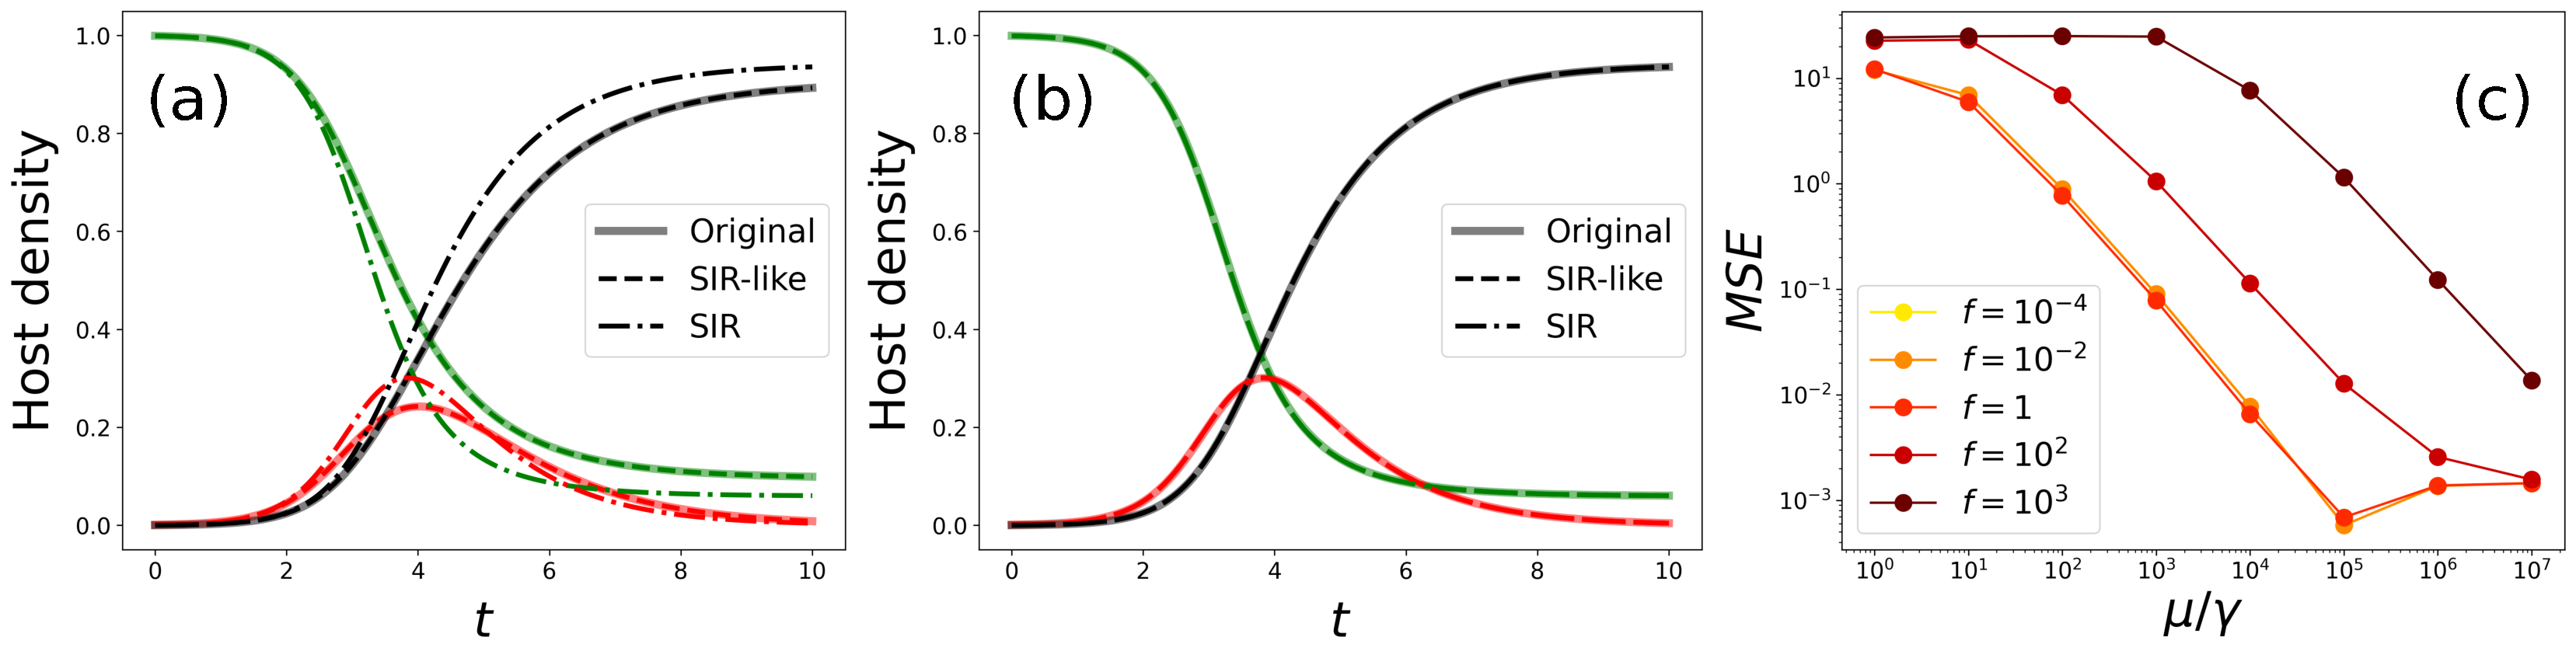
\includegraphics[width=\textwidth]{Figures/SIR_like_approx_comp.pdf}
    \caption[Comparison between the original model and the
    reductions]{Comparison between the original model and the reductions,
    \cref{eq:SIR_like} (SIR-like) and \cref{eq:SIR} (SIR) with $N=100$,
    $\mu/\gamma=10^{3}$ and $f=1$. $\beta$ was chosen such that $R_0=3$.  (a)
    $\lambda=1$, (b) $\lambda=10^3$, (c) Mean Squared Error between the
    original
    model and the SIR approximations as function of the ratio $\mu/\gamma$ and
    $f$.}
    \label{fig:SIR_like_approx}
\end{figure}

In \cref{fig:SIR_like_approx} we show the validity of the reduced models
\cref{eq:SIR_like} and \cref{eq:SIR}. \cref{fig:SIR_like_approx}(a) shows that
the SIR-like model (\cref{eq:SIR_like}) works when the time-scale approximation
can be performed (as $\mu/\gamma\gg1$) but the SIR model fails when the
condition $\lambda N_H \gg I_H$ is not fulfilled. Conversely, in
\cref{fig:SIR_like_approx}(b) we show that as $\lambda N_H \gg I_H$ is
fulfilled, then the SIR model perfectly matches the original model. Finally,
\cref{fig:SIR_like_approx}(c) shows the decrease in the mean squared error of
the approximation as the condition \cref{eq:timescales_condition} is fulfilled
for different values of $f$.

\section{Conclusions}\label{sec:conclusions}

In the present work we have analyzed several features of a compartmental
deterministic model for vector-borne diseases with $3$ compartments for hosts
and $2$ for vectors, that does not consider neither direct host to host nor
vertical transmission. The goal is to study the behavior of the model in the
case that the vector population is not stationary. In this case, the
pre-pandemic disease-free state is not a fixed point (equilibrium state) of the
dynamical system, and, in principle, the methods that are customarily used to
determine the basic reproduction number, $R_0$ do not work. This is so because
these methods determine the onset of an outbreak by performing a linear
stability analysis of the disease-free state, assuming that it is a fixed point
of the model. A common assumption made in the literature is to determine $R_0$
from the asymptotic state for the vectors (if it is not an extinction state), a
fixed point of the model.

We have analyzed several initial conditions of the vector population,
characterizing different regimes. In the case that the initial condition for
the number of vectors is below the asymptotic state, implying that the vector
population overall grows, then $R_0$ as determined from the asymptotic state
correctly predicts the existence (or not) of an epidemic outbreak, but with a
temporal delay in its appearance. This result contrasts with the situation in
which the initial state is above the asymptotic state, with an overall decrease
in the vector population. In this case $R_0$ determined from the asymptotic
state may fail badly, predicting no outbreak while a large fraction of the
population might get infected. We present a simple, albeit useful,
generalization of $R_0$ that is able to give a reasonable prediction of the
epidemic threshold for decaying populations, including the case in which
vectors become extinct, a case in which the asymptotic estimation to determine
$R_0$ cannot be applied.

Compartmental models of vector-borne diseases usually have many
compartments and parameters, which can lead to a problem of parameter
unidentifiability. The model analyzed here is not an exception, and when
applied to real-world cases many different combinations of the parameters could
be able to reproduce the available data. Thus, in order to facilitate the
application of the model to experimental data, we have studied a useful
fast-slow (or adiabatic) approximation that allows to reduce the model if the
parameters fulfil certain conditions. In particular, our study shows that
under quite realistic assumptions (the typical timescale of hosts infection and
death is much slower than vector timescales) it is possible to obtain a reduced
SIR model. We recall that this reduction implies that, under these assumptions,
the process by which hosts (that could be immobile) get infected through the
action of vectors is equivalent to a direct interaction among hosts.

The deterministic compartmental model analyzed here, with some
modifications, is a clear candidate to study many vector-borne diseases, in
particular phytopathologies. Furthermore, in case of parameter
unidientifiability the model reductions performed in this work could be useful
to solve this issue. In any case, this description is still idealized, as
compartmental models imply a well-mixed assumption in which space is not
explicitly described. This kind of representations are not always applicable to
real-world scenarios although are useful as a first approximation. Thus, future
research should focus on the integration of space and vector mobility in the
model to account for more realistic situations.